\documentclass[12pt,a4paper]{article}
\usepackage[utf8]{vietnam}
\usepackage{amsmath,amssymb}
\usepackage{tabularx}
\usepackage{tikz}
\usepackage{xcolor}
\usepackage[top=0.6cm, bottom=0.6cm, left=0.6cm, right=0.6cm]{geometry}
\usepackage[dethi]{ex_test}

\SAOPTN{widthSA=2.6,heightSA=0.62}
\setlength{\parskip}{0pt}

% Dòng kẻ chấm mờ chuẩn viết tay
\newcommand{\dongke}[1]{%
  \begingroup%
  \setlength{\parskip}{0pt}%
  \baselineskip=18.5pt%
  \vspace{1.0mm}%
  \foreach \i in {1,...,#1}{%
    \noindent{\color{gray!60}\dotfill}\par%
  }%
  \vspace{0.6mm}%
  \endgroup%
}

% Khu vực bài làm chia 2 cột có vách ngăn mờ ở giữa
\newcommand{\dongkeHaiCot}[1]{%
  \par\vspace{0.5mm}%
  \noindent%
  \begin{minipage}[t]{0.485\linewidth}%
    \dongke{#1}%
  \end{minipage}%
  \hfill%
  {\color{gray!60}\vrule}%
  \hfill%
  \begin{minipage}[t]{0.485\linewidth}%
    \dongke{#1}%
  \end{minipage}%
}

% Định nghĩa ô bài tập tự luận trong bảng
\newcommand{\oBaiTap}[3][5]{%
  \vspace{1.0mm}%
  \noindent\textbf{#2} #3\par%
  \dongke{#1}%
}

\begin{document}
\pagestyle{empty}
% =============================================================================
% ========================= MA DE 101 - MAT TRUOC (TRANG 1/2) =============
% =============================================================================
\noindent
\begin{tabularx}{\linewidth}{|X|c|}
\hline
\textbf{PHIẾU KIỂM TRA ĐỊNH KỲ TOÁN 7 - TUẦN 12 - BUỔI 01} & \textbf{Mã đề: 101 - Trang 1/2} \\
\hline
\end{tabularx}

\vspace{1.0mm}

\noindent
\begin{tabularx}{\linewidth}{|p{3.2cm}|X|}
\hline
\centering\textbf{ĐIỂM SỐ} & \centering\textbf{LỜI NHẬN XÉT CỦA THẦY CÔ} \tabularnewline
\hline
\rule{0pt}{1.8cm} & \tabularnewline
\hline
\end{tabularx}

\vspace{1.2mm}
\noindent\textbf{Câu 1 (0,25 điểm).} $\triangle ABC$ cân tại $A, \widehat{A} = 50^\circ$. Tính: $\widehat{B} =$ \shortans{65^\circ}\par\vspace{2.5mm}
\noindent\textbf{Câu 2 (0,25 điểm).} $\triangle MNP$ cân tại $M, \widehat{N} = 70^\circ$. Tính: $\widehat{M} =$ \shortans{40^\circ}\par\vspace{2.5mm}
\noindent\textbf{Câu 3 (0,25 điểm).} $\triangle ABC$ vuông cân tại $A$. Số đo góc $B$ là: \shortans{45^\circ}\par\vspace{2.5mm}
\noindent\textbf{Câu 4 (0,25 điểm).} $\triangle ABC$ cân tại $A, \widehat{B} = 60^\circ$. $\triangle ABC$ là tam giác gì? \shortans{Tam giác đều}\par\vspace{2.5mm}
\noindent\textbf{Câu 5 (0,25 điểm).} $\triangle ABC$ cân tại $A, AB = 7\text{ cm}, BC = 5\text{ cm}$. Chu vi là: \shortans{19\text{ cm}}\par\vspace{2.5mm}
\noindent\textbf{Câu 6 (0,25 điểm).} Giá trị của $\sqrt{121} =$ \shortans{11}\par\vspace{2.5mm}
\noindent\textbf{Câu 7 (0,25 điểm).} Tính giá trị: $|-4{,}5| + |1{,}5| =$ \shortans{6}\par\vspace{2.5mm}
\noindent\textbf{Câu 8 (0,25 điểm).} Tính giá trị: $\left(-\dfrac{1}{3}\right)^3 =$ \shortans{-\dfrac{1}{27}}\par\vspace{2.5mm}
\noindent\textbf{Câu 9 (0,25 điểm).} Mái nhà tam giác cân có góc đỉnh $110^\circ$. Góc dốc của mái là: \shortans{35^\circ}\par\vspace{2.5mm}
\noindent\textbf{Câu 10 (0,25 điểm).} $\triangle ABC$ có $\widehat{A} = 70^\circ, \widehat{B} = 40^\circ$. $\triangle ABC$ cân tại đâu? \shortans{Đỉnh B}\par\vspace{2.5mm}
\vspace{0.2mm}
\noindent\textbf{Câu 11 (3,0 điểm). Thực hiện phép tính (hợp lý nếu có thể):}
\vspace{0.5mm}

\noindent
\begin{tabularx}{\linewidth}{|X|X|}
\hline
\oBaiTap[5]{a) (0,5 điểm)}{$\dfrac{5}{9} + \left(-\dfrac{7}{11}\right) + \dfrac{4}{9} + \left(-\dfrac{4}{11}\right)$} & 
\oBaiTap[5]{b) (0,5 điểm)}{$\dfrac{5}{7} \cdot \left(-\dfrac{8}{13}\right) + \dfrac{5}{7} \cdot \left(-\dfrac{5}{13}\right)$} \\
\hline
\oBaiTap[5]{c) (0,5 điểm)}{$\sqrt{\dfrac{49}{25}} - \left(-\dfrac{1}{2}\right)^2 : \dfrac{5}{4}$} & 
\oBaiTap[5]{d) (0,5 điểm)}{$\dfrac{3}{4} - \left[\dfrac{1}{2} - \left(\dfrac{2}{3} - \dfrac{1}{6}\right)\right]$} \\
\hline
\oBaiTap[5]{e) (0,5 điểm)}{$\left|-\dfrac{3}{4}\right| : \dfrac{3}{2} + \sqrt{\dfrac{1}{16}} - 0{,}75$} & 
\oBaiTap[5]{f) (0,5 điểm)}{$\dfrac{4^3 \cdot 9^2}{2^5 \cdot 3^3}$} \\
\hline
\end{tabularx}

\newpage
% =============================================================================
% ========================= MA DE 101 - MAT SAU (TRANG 2/2) ==============
% =============================================================================
\noindent
\begin{tabularx}{\linewidth}{|X|}
\hline
\centering\textbf{TOÁN 7 - TUẦN 12 - BUỔI 01 | Mã đề: 101 - Trang 2/2} \\
\hline
\end{tabularx}

\vspace{1.2mm}

\noindent\textbf{Câu 12 (2,0 điểm). Tìm số hữu tỉ $x$, biết:}
\vspace{0.5mm}

\noindent
\begin{tabularx}{\linewidth}{|X|X|}
\hline
\oBaiTap[5]{a) (0,5 điểm)}{$x - \dfrac{3}{5} = -\dfrac{1}{2}$} & 
\oBaiTap[5]{b) (0,5 điểm)}{$\dfrac{2}{3}x + \dfrac{1}{2} = -\dfrac{5}{6}$} \\
\hline
\oBaiTap[5]{c) (0,5 điểm)}{$\left|x - \dfrac{1}{3}\right| = \dfrac{2}{3}$} & 
\oBaiTap[5]{d) (0,5 điểm)}{$\left(x + \dfrac{1}{2}\right)^2 = \dfrac{9}{16}$} \\
\hline
\end{tabularx}

\vspace{1.2mm}

\noindent
\begin{tabularx}{\linewidth}{|X|}
\hline
\vspace{0.5mm}
\begin{minipage}[t]{0.62\linewidth}
\vspace{0pt}
\textbf{Câu 13 (2,0 điểm).} Cho tam giác $ABC$ cân tại $A$ ($\widehat{A} < 90^\circ$). Gọi $H$ là trung điểm của cạnh $BC$.\par\vspace{0.3mm}
\textbf{a) (1,0 điểm)} Chứng minh $\triangle ABH = \triangle ACH$. Suy ra $AH \perp BC$ và $AH$ là phân giác $\widehat{BAC}$.\par\vspace{0.3mm}
\textbf{b) (1,0 điểm)} Từ $H$ kẻ $HM \perp AB$ ($M \in AB$), $HN \perp AC$ ($N \in AC$). Chứng minh $HM = HN$ và $\triangle HMN$ cân.
\end{minipage}\hfill
\begin{minipage}[t]{0.36\linewidth}
\vspace{0pt}\centering
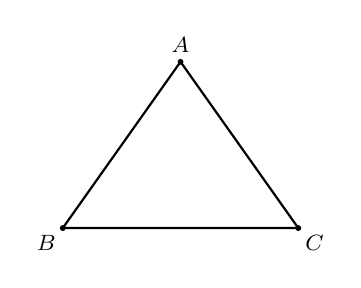
\begin{tikzpicture}[scale=0.88, line cap=round, line join=round, >=stealth, font=\footnotesize]
  \coordinate (A) at (0, 2.4);
  \coordinate (B) at (-1.7, 0);
  \coordinate (C) at (1.7, 0);

  \draw[thick] (A) -- (B) -- (C) -- cycle;

  \fill (A) circle (1.2pt) node[above] {$A$};
  \fill (B) circle (1.2pt) node[below left=-1pt] {$B$};
  \fill (C) circle (1.2pt) node[below right=-1pt] {$C$};
\end{tikzpicture}
\end{minipage}\par
\vspace{0.4mm}
\noindent\textit{Bài giải:}\dongkeHaiCot{10}
\\ \hline
\end{tabularx}

\vspace{1.2mm}

\noindent
\begin{tabularx}{\linewidth}{|X|}
\hline
\vspace{0.5mm}
\textbf{Câu 14 (0,5 điểm).} Tìm giá trị lớn nhất của biểu thức: $A = \dfrac{12}{|x - 3| + 4}$ với $x \in \mathbb{R}$.\par
\vspace{0.4mm}
\noindent\textit{Bài giải:}\dongkeHaiCot{6}
\\ \hline
\end{tabularx}

\newpage
% =============================================================================
% ========================= MA DE 102 - MAT TRUOC (TRANG 1/2) =============
% =============================================================================
\noindent
\begin{tabularx}{\linewidth}{|X|c|}
\hline
\textbf{PHIẾU KIỂM TRA ĐỊNH KỲ TOÁN 7 - TUẦN 12 - BUỔI 01} & \textbf{Mã đề: 102 - Trang 1/2} \\
\hline
\end{tabularx}

\vspace{1.0mm}

\noindent
\begin{tabularx}{\linewidth}{|p{3.2cm}|X|}
\hline
\centering\textbf{ĐIỂM SỐ} & \centering\textbf{LỜI NHẬN XÉT CỦA THẦY CÔ} \tabularnewline
\hline
\rule{0pt}{1.8cm} & \tabularnewline
\hline
\end{tabularx}

\vspace{1.2mm}
\noindent\textbf{Câu 1 (0,25 điểm).} $\triangle ABC$ cân tại $A, \widehat{A} = 70^\circ$. Tính: $\widehat{B} =$ \shortans{55^\circ}\par\vspace{2.5mm}
\noindent\textbf{Câu 2 (0,25 điểm).} $\triangle MNP$ cân tại $M, \widehat{N} = 65^\circ$. Tính: $\widehat{M} =$ \shortans{50^\circ}\par\vspace{2.5mm}
\noindent\textbf{Câu 3 (0,25 điểm).} $\triangle MNP$ vuông cân tại $M$. Số đo góc $N$ là: \shortans{45^\circ}\par\vspace{2.5mm}
\noindent\textbf{Câu 4 (0,25 điểm).} $\triangle MNP$ cân tại $M, \widehat{M} = 60^\circ$. $\triangle MNP$ là tam giác gì? \shortans{Tam giác đều}\par\vspace{2.5mm}
\noindent\textbf{Câu 5 (0,25 điểm).} $\triangle ABC$ cân tại $A, AB = 8\text{ cm}, BC = 6\text{ cm}$. Chu vi là: \shortans{22\text{ cm}}\par\vspace{2.5mm}
\noindent\textbf{Câu 6 (0,25 điểm).} Giá trị của $\sqrt{144} =$ \shortans{12}\par\vspace{2.5mm}
\noindent\textbf{Câu 7 (0,25 điểm).} Tính giá trị: $|-5{,}2| + |2{,}8| =$ \shortans{8}\par\vspace{2.5mm}
\noindent\textbf{Câu 8 (0,25 điểm).} Tính giá trị: $\left(-\dfrac{1}{2}\right)^4 =$ \shortans{\dfrac{1}{16}}\par\vspace{2.5mm}
\noindent\textbf{Câu 9 (0,25 điểm).} Mái nhà tam giác cân có góc đỉnh $100^\circ$. Góc dốc của mái là: \shortans{40^\circ}\par\vspace{2.5mm}
\noindent\textbf{Câu 10 (0,25 điểm).} $\triangle ABC$ có $\widehat{B} = 50^\circ, \widehat{C} = 80^\circ$. $\triangle ABC$ cân tại đâu? \shortans{Đỉnh C}\par\vspace{2.5mm}
\vspace{0.2mm}
\noindent\textbf{Câu 11 (3,0 điểm). Thực hiện phép tính (hợp lý nếu có thể):}
\vspace{0.5mm}

\noindent
\begin{tabularx}{\linewidth}{|X|X|}
\hline
\oBaiTap[5]{a) (0,5 điểm)}{$\dfrac{7}{12} + \left(-\dfrac{5}{8}\right) + \dfrac{5}{12} + \left(-\dfrac{3}{8}\right)$} & 
\oBaiTap[5]{b) (0,5 điểm)}{$\dfrac{4}{9} \cdot \left(-\dfrac{11}{17}\right) + \dfrac{4}{9} \cdot \left(-\dfrac{6}{17}\right)$} \\
\hline
\oBaiTap[5]{c) (0,5 điểm)}{$\sqrt{\dfrac{64}{25}} - \left(-\dfrac{1}{3}\right)^2 : \dfrac{5}{9}$} & 
\oBaiTap[5]{d) (0,5 điểm)}{$\dfrac{5}{6} - \left[\dfrac{2}{3} - \left(\dfrac{3}{4} - \dfrac{1}{12}\right)\right]$} \\
\hline
\oBaiTap[5]{e) (0,5 điểm)}{$\left|-\dfrac{2}{3}\right| : \dfrac{4}{3} + \sqrt{\dfrac{1}{4}} - 1{,}0$} & 
\oBaiTap[5]{f) (0,5 điểm)}{$\dfrac{8^2 \cdot 9^3}{2^5 \cdot 3^5}$} \\
\hline
\end{tabularx}

\newpage
% =============================================================================
% ========================= MA DE 102 - MAT SAU (TRANG 2/2) ==============
% =============================================================================
\noindent
\begin{tabularx}{\linewidth}{|X|}
\hline
\centering\textbf{TOÁN 7 - TUẦN 12 - BUỔI 01 | Mã đề: 102 - Trang 2/2} \\
\hline
\end{tabularx}

\vspace{1.2mm}

\noindent\textbf{Câu 12 (2,0 điểm). Tìm số hữu tỉ $x$, biết:}
\vspace{0.5mm}

\noindent
\begin{tabularx}{\linewidth}{|X|X|}
\hline
\oBaiTap[5]{a) (0,5 điểm)}{$x - \dfrac{2}{3} = -\dfrac{1}{4}$} & 
\oBaiTap[5]{b) (0,5 điểm)}{$\dfrac{3}{4}x + \dfrac{1}{3} = -\dfrac{5}{12}$} \\
\hline
\oBaiTap[5]{c) (0,5 điểm)}{$\left|x - \dfrac{1}{2}\right| = \dfrac{3}{4}$} & 
\oBaiTap[5]{d) (0,5 điểm)}{$\left(x + \dfrac{1}{3}\right)^2 = \dfrac{4}{9}$} \\
\hline
\end{tabularx}

\vspace{1.2mm}

\noindent
\begin{tabularx}{\linewidth}{|X|}
\hline
\vspace{0.5mm}
\begin{minipage}[t]{0.62\linewidth}
\vspace{0pt}
\textbf{Câu 13 (2,0 điểm).} Cho tam giác $MNP$ cân tại $M$ ($\widehat{M} < 90^\circ$). Gọi $I$ là trung điểm của cạnh $NP$.\par\vspace{0.3mm}
\textbf{a) (1,0 điểm)} Chứng minh $\triangle MNI = \triangle MPI$. Suy ra $MI \perp NP$ và $MI$ là phân giác $\widehat{NMP}$.\par\vspace{0.3mm}
\textbf{b) (1,0 điểm)} Từ $I$ kẻ $IE \perp MN$ ($E \in MN$), $IF \perp MP$ ($F \in MP$). Chứng minh $IE = IF$ và $\triangle IEF$ cân.
\end{minipage}\hfill
\begin{minipage}[t]{0.36\linewidth}
\vspace{0pt}\centering
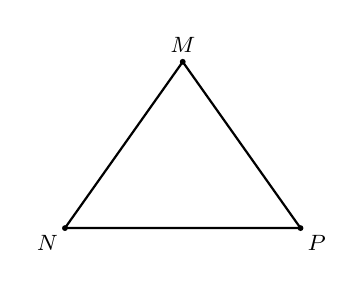
\begin{tikzpicture}[scale=0.88, line cap=round, line join=round, >=stealth, font=\footnotesize]
  \coordinate (M) at (0, 2.4);
  \coordinate (N) at (-1.7, 0);
  \coordinate (P) at (1.7, 0);

  \draw[thick] (M) -- (N) -- (P) -- cycle;

  \fill (M) circle (1.2pt) node[above] {$M$};
  \fill (N) circle (1.2pt) node[below left=-1pt] {$N$};
  \fill (P) circle (1.2pt) node[below right=-1pt] {$P$};
\end{tikzpicture}
\end{minipage}\par
\vspace{0.4mm}
\noindent\textit{Bài giải:}\dongkeHaiCot{10}
\\ \hline
\end{tabularx}

\vspace{1.2mm}

\noindent
\begin{tabularx}{\linewidth}{|X|}
\hline
\vspace{0.5mm}
\textbf{Câu 14 (0,5 điểm).} Tìm giá trị lớn nhất của biểu thức: $B = \dfrac{15}{|x - 2| + 5}$ với $x \in \mathbb{R}$.\par
\vspace{0.4mm}
\noindent\textit{Bài giải:}\dongkeHaiCot{6}
\\ \hline
\end{tabularx}

\newpage
% =============================================================================
% ========================= MA DE 103 - MAT TRUOC (TRANG 1/2) =============
% =============================================================================
\noindent
\begin{tabularx}{\linewidth}{|X|c|}
\hline
\textbf{PHIẾU KIỂM TRA ĐỊNH KỲ TOÁN 7 - TUẦN 12 - BUỔI 01} & \textbf{Mã đề: 103 - Trang 1/2} \\
\hline
\end{tabularx}

\vspace{1.0mm}

\noindent
\begin{tabularx}{\linewidth}{|p{3.2cm}|X|}
\hline
\centering\textbf{ĐIỂM SỐ} & \centering\textbf{LỜI NHẬN XÉT CỦA THẦY CÔ} \tabularnewline
\hline
\rule{0pt}{1.8cm} & \tabularnewline
\hline
\end{tabularx}

\vspace{1.2mm}
\noindent\textbf{Câu 1 (0,25 điểm).} $\triangle ABC$ cân tại $A, \widehat{A} = 40^\circ$. Tính: $\widehat{B} =$ \shortans{70^\circ}\par\vspace{2.5mm}
\noindent\textbf{Câu 2 (0,25 điểm).} $\triangle MNP$ cân tại $M, \widehat{N} = 55^\circ$. Tính: $\widehat{M} =$ \shortans{70^\circ}\par\vspace{2.5mm}
\noindent\textbf{Câu 3 (0,25 điểm).} $\triangle DEF$ vuông cân tại $D$. Số đo góc $E$ là: \shortans{45^\circ}\par\vspace{2.5mm}
\noindent\textbf{Câu 4 (0,25 điểm).} $\triangle DEF$ có $\widehat{D} = \widehat{E} = 60^\circ$. $\triangle DEF$ là tam giác gì? \shortans{Tam giác đều}\par\vspace{2.5mm}
\noindent\textbf{Câu 5 (0,25 điểm).} $\triangle ABC$ cân tại $A, AB = 9\text{ cm}, BC = 4\text{ cm}$. Chu vi là: \shortans{22\text{ cm}}\par\vspace{2.5mm}
\noindent\textbf{Câu 6 (0,25 điểm).} Giá trị của $\sqrt{169} =$ \shortans{13}\par\vspace{2.5mm}
\noindent\textbf{Câu 7 (0,25 điểm).} Tính giá trị: $|-3{,}8| + |4{,}2| =$ \shortans{8}\par\vspace{2.5mm}
\noindent\textbf{Câu 8 (0,25 điểm).} Tính giá trị: $\left(-\dfrac{2}{3}\right)^3 =$ \shortans{-\dfrac{8}{27}}\par\vspace{2.5mm}
\noindent\textbf{Câu 9 (0,25 điểm).} Thang chữ A tam giác cân có góc đỉnh $40^\circ$. Góc chân thang là: \shortans{70^\circ}\par\vspace{2.5mm}
\noindent\textbf{Câu 10 (0,25 điểm).} $\triangle ABC$ có $\widehat{A} = 80^\circ, \widehat{B} = 50^\circ$. $\triangle ABC$ cân tại đâu? \shortans{Đỉnh A}\par\vspace{2.5mm}
\vspace{0.2mm}
\noindent\textbf{Câu 11 (3,0 điểm). Thực hiện phép tính (hợp lý nếu có thể):}
\vspace{0.5mm}

\noindent
\begin{tabularx}{\linewidth}{|X|X|}
\hline
\oBaiTap[5]{a) (0,5 điểm)}{$\dfrac{4}{13} + \left(-\dfrac{7}{9}\right) + \dfrac{9}{13} + \left(-\dfrac{2}{9}\right)$} & 
\oBaiTap[5]{b) (0,5 điểm)}{$\dfrac{6}{11} \cdot \left(-\dfrac{9}{14}\right) + \dfrac{6}{11} \cdot \left(-\dfrac{5}{14}\right)$} \\
\hline
\oBaiTap[5]{c) (0,5 điểm)}{$\sqrt{\dfrac{36}{25}} - \left(-\dfrac{1}{2}\right)^2 : \dfrac{5}{4}$} & 
\oBaiTap[5]{d) (0,5 điểm)}{$\dfrac{7}{8} - \left[\dfrac{3}{4} - \left(\dfrac{5}{6} - \dfrac{1}{12}\right)\right]$} \\
\hline
\oBaiTap[5]{e) (0,5 điểm)}{$\left|-\dfrac{4}{5}\right| : \dfrac{8}{5} + \sqrt{\dfrac{1}{4}} - 1{,}0$} & 
\oBaiTap[5]{f) (0,5 điểm)}{$\dfrac{4^4 \cdot 27^2}{2^7 \cdot 3^5}$} \\
\hline
\end{tabularx}

\newpage
% =============================================================================
% ========================= MA DE 103 - MAT SAU (TRANG 2/2) ==============
% =============================================================================
\noindent
\begin{tabularx}{\linewidth}{|X|}
\hline
\centering\textbf{TOÁN 7 - TUẦN 12 - BUỔI 01 | Mã đề: 103 - Trang 2/2} \\
\hline
\end{tabularx}

\vspace{1.2mm}

\noindent\textbf{Câu 12 (2,0 điểm). Tìm số hữu tỉ $x$, biết:}
\vspace{0.5mm}

\noindent
\begin{tabularx}{\linewidth}{|X|X|}
\hline
\oBaiTap[5]{a) (0,5 điểm)}{$x - \dfrac{3}{4} = -\dfrac{1}{3}$} & 
\oBaiTap[5]{b) (0,5 điểm)}{$\dfrac{4}{5}x + \dfrac{1}{2} = -\dfrac{3}{10}$} \\
\hline
\oBaiTap[5]{c) (0,5 điểm)}{$\left|x - \dfrac{2}{5}\right| = \dfrac{3}{5}$} & 
\oBaiTap[5]{d) (0,5 điểm)}{$\left(x + \dfrac{1}{4}\right)^2 = \dfrac{25}{16}$} \\
\hline
\end{tabularx}

\vspace{1.2mm}

\noindent
\begin{tabularx}{\linewidth}{|X|}
\hline
\vspace{0.5mm}
\begin{minipage}[t]{0.62\linewidth}
\vspace{0pt}
\textbf{Câu 13 (2,0 điểm).} Cho tam giác $DEF$ cân tại $D$ ($\widehat{D} < 90^\circ$). Gọi $K$ là trung điểm của cạnh $EF$.\par\vspace{0.3mm}
\textbf{a) (1,0 điểm)} Chứng minh $\triangle DEK = \triangle DFK$. Suy ra $DK \perp EF$ và $DK$ là phân giác $\widehat{EDF}$.\par\vspace{0.3mm}
\textbf{b) (1,0 điểm)} Từ $K$ kẻ $KP \perp DE$ ($P \in DE$), $KQ \perp DF$ ($Q \in DF$). Chứng minh $KP = KQ$ và $\triangle KPQ$ cân.
\end{minipage}\hfill
\begin{minipage}[t]{0.36\linewidth}
\vspace{0pt}\centering
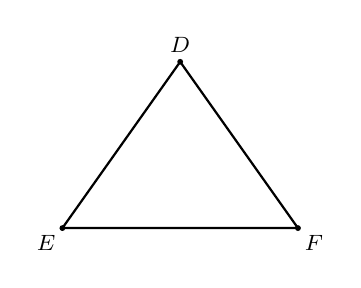
\begin{tikzpicture}[scale=0.88, line cap=round, line join=round, >=stealth, font=\footnotesize]
  \coordinate (D) at (0, 2.4);
  \coordinate (E) at (-1.7, 0);
  \coordinate (F) at (1.7, 0);

  \draw[thick] (D) -- (E) -- (F) -- cycle;

  \fill (D) circle (1.2pt) node[above] {$D$};
  \fill (E) circle (1.2pt) node[below left=-1pt] {$E$};
  \fill (F) circle (1.2pt) node[below right=-1pt] {$F$};
\end{tikzpicture}
\end{minipage}\par
\vspace{0.4mm}
\noindent\textit{Bài giải:}\dongkeHaiCot{10}
\\ \hline
\end{tabularx}

\vspace{1.2mm}

\noindent
\begin{tabularx}{\linewidth}{|X|}
\hline
\vspace{0.5mm}
\textbf{Câu 14 (0,5 điểm).} Tìm giá trị lớn nhất của biểu thức: $C = \dfrac{18}{|x - 4| + 6}$ với $x \in \mathbb{R}$.\par
\vspace{0.4mm}
\noindent\textit{Bài giải:}\dongkeHaiCot{6}
\\ \hline
\end{tabularx}

\newpage
% =============================================================================
% ========================= MA DE 104 - MAT TRUOC (TRANG 1/2) =============
% =============================================================================
\noindent
\begin{tabularx}{\linewidth}{|X|c|}
\hline
\textbf{PHIẾU KIỂM TRA ĐỊNH KỲ TOÁN 7 - TUẦN 12 - BUỔI 01} & \textbf{Mã đề: 104 - Trang 1/2} \\
\hline
\end{tabularx}

\vspace{1.0mm}

\noindent
\begin{tabularx}{\linewidth}{|p{3.2cm}|X|}
\hline
\centering\textbf{ĐIỂM SỐ} & \centering\textbf{LỜI NHẬN XÉT CỦA THẦY CÔ} \tabularnewline
\hline
\rule{0pt}{1.8cm} & \tabularnewline
\hline
\end{tabularx}

\vspace{1.2mm}
\noindent\textbf{Câu 1 (0,25 điểm).} $\triangle ABC$ cân tại $A, \widehat{A} = 80^\circ$. Tính: $\widehat{B} =$ \shortans{50^\circ}\par\vspace{2.5mm}
\noindent\textbf{Câu 2 (0,25 điểm).} $\triangle MNP$ cân tại $M, \widehat{N} = 75^\circ$. Tính: $\widehat{M} =$ \shortans{30^\circ}\par\vspace{2.5mm}
\noindent\textbf{Câu 3 (0,25 điểm).} $\triangle HIK$ vuông cân tại $H$. Số đo góc $I$ là: \shortans{45^\circ}\par\vspace{2.5mm}
\noindent\textbf{Câu 4 (0,25 điểm).} $\triangle ABC$ có $AB = BC = CA = 5\text{ cm}$. Số đo góc $A$ là: \shortans{60^\circ}\par\vspace{2.5mm}
\noindent\textbf{Câu 5 (0,25 điểm).} $\triangle ABC$ cân tại $A, AB = 6\text{ cm}, BC = 7\text{ cm}$. Chu vi là: \shortans{19\text{ cm}}\par\vspace{2.5mm}
\noindent\textbf{Câu 6 (0,25 điểm).} Giá trị của $\sqrt{196} =$ \shortans{14}\par\vspace{2.5mm}
\noindent\textbf{Câu 7 (0,25 điểm).} Tính giá trị: $|-6{,}4| + |1{,}6| =$ \shortans{8}\par\vspace{2.5mm}
\noindent\textbf{Câu 8 (0,25 điểm).} Tính giá trị: $\left(-\dfrac{1}{2}\right)^5 =$ \shortans{-\dfrac{1}{32}}\par\vspace{2.5mm}
\noindent\textbf{Câu 9 (0,25 điểm).} Thang chữ A tam giác cân có góc đỉnh $50^\circ$. Góc chân thang là: \shortans{65^\circ}\par\vspace{2.5mm}
\noindent\textbf{Câu 10 (0,25 điểm).} $\triangle ABC$ có $\widehat{A} = 40^\circ, \widehat{C} = 70^\circ$. $\triangle ABC$ cân tại đâu? \shortans{Đỉnh A}\par\vspace{2.5mm}
\vspace{0.2mm}
\noindent\textbf{Câu 11 (3,0 điểm). Thực hiện phép tính (hợp lý nếu có thể):}
\vspace{0.5mm}

\noindent
\begin{tabularx}{\linewidth}{|X|X|}
\hline
\oBaiTap[5]{a) (0,5 điểm)}{$\dfrac{8}{15} + \left(-\dfrac{3}{7}\right) + \dfrac{7}{15} + \left(-\dfrac{4}{7}\right)$} & 
\oBaiTap[5]{b) (0,5 điểm)}{$\dfrac{7}{15} \cdot \left(-\dfrac{12}{19}\right) + \dfrac{7}{15} \cdot \left(-\dfrac{7}{19}\right)$} \\
\hline
\oBaiTap[5]{c) (0,5 điểm)}{$\sqrt{\dfrac{16}{9}} - \left(-\dfrac{1}{2}\right)^2 : \dfrac{3}{4}$} & 
\oBaiTap[5]{d) (0,5 điểm)}{$\dfrac{4}{5} - \left[\dfrac{1}{2} - \left(\dfrac{5}{6} - \dfrac{1}{3}\right)\right]$} \\
\hline
\oBaiTap[5]{e) (0,5 điểm)}{$\left|-\dfrac{5}{6}\right| : \dfrac{5}{3} + \sqrt{\dfrac{1}{4}} - 1{,}0$} & 
\oBaiTap[5]{f) (0,5 điểm)}{$\dfrac{16^2 \cdot 9^3}{2^7 \cdot 3^5}$} \\
\hline
\end{tabularx}

\newpage
% =============================================================================
% ========================= MA DE 104 - MAT SAU (TRANG 2/2) ==============
% =============================================================================
\noindent
\begin{tabularx}{\linewidth}{|X|}
\hline
\centering\textbf{TOÁN 7 - TUẦN 12 - BUỔI 01 | Mã đề: 104 - Trang 2/2} \\
\hline
\end{tabularx}

\vspace{1.2mm}

\noindent\textbf{Câu 12 (2,0 điểm). Tìm số hữu tỉ $x$, biết:}
\vspace{0.5mm}

\noindent
\begin{tabularx}{\linewidth}{|X|X|}
\hline
\oBaiTap[5]{a) (0,5 điểm)}{$x - \dfrac{4}{5} = -\dfrac{1}{2}$} & 
\oBaiTap[5]{b) (0,5 điểm)}{$\dfrac{3}{5}x + \dfrac{1}{4} = -\dfrac{7}{20}$} \\
\hline
\oBaiTap[5]{c) (0,5 điểm)}{$\left|x - \dfrac{1}{4}\right| = \dfrac{3}{4}$} & 
\oBaiTap[5]{d) (0,5 điểm)}{$\left(x + \dfrac{1}{5}\right)^2 = \dfrac{9}{25}$} \\
\hline
\end{tabularx}

\vspace{1.2mm}

\noindent
\begin{tabularx}{\linewidth}{|X|}
\hline
\vspace{0.5mm}
\begin{minipage}[t]{0.62\linewidth}
\vspace{0pt}
\textbf{Câu 13 (2,0 điểm).} Cho tam giác $ABC$ cân tại $A$ ($\widehat{A} < 90^\circ$). Gọi $M$ là trung điểm của cạnh $BC$.\par\vspace{0.3mm}
\textbf{a) (1,0 điểm)} Chứng minh $\triangle ABM = \triangle ACM$. Suy ra $AM \perp BC$ và $AM$ là phân giác $\widehat{BAC}$.\par\vspace{0.3mm}
\textbf{b) (1,0 điểm)} Từ $M$ kẻ $ME \perp AB$ ($E \in AB$), $MF \perp AC$ ($F \in AC$). Chứng minh $ME = MF$ và $\triangle MEF$ cân.
\end{minipage}\hfill
\begin{minipage}[t]{0.36\linewidth}
\vspace{0pt}\centering
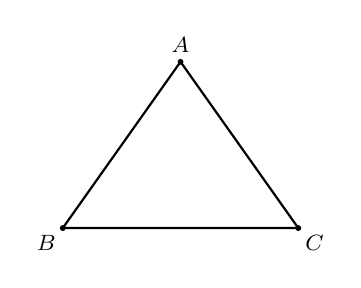
\begin{tikzpicture}[scale=0.88, line cap=round, line join=round, >=stealth, font=\footnotesize]
  \coordinate (A) at (0, 2.4);
  \coordinate (B) at (-1.7, 0);
  \coordinate (C) at (1.7, 0);

  \draw[thick] (A) -- (B) -- (C) -- cycle;

  \fill (A) circle (1.2pt) node[above] {$A$};
  \fill (B) circle (1.2pt) node[below left=-1pt] {$B$};
  \fill (C) circle (1.2pt) node[below right=-1pt] {$C$};
\end{tikzpicture}
\end{minipage}\par
\vspace{0.4mm}
\noindent\textit{Bài giải:}\dongkeHaiCot{10}
\\ \hline
\end{tabularx}

\vspace{1.2mm}

\noindent
\begin{tabularx}{\linewidth}{|X|}
\hline
\vspace{0.5mm}
\textbf{Câu 14 (0,5 điểm).} Tìm giá trị lớn nhất của biểu thức: $D = \dfrac{20}{|x - 5| + 4}$ với $x \in \mathbb{R}$.\par
\vspace{0.4mm}
\noindent\textit{Bài giải:}\dongkeHaiCot{6}
\\ \hline
\end{tabularx}
\end{document}
